%----------------------------------------------------------------------------------------
%	PACKAGES AND OTHER DOCUMENT CONFIGURATIONS
%----------------------------------------------------------------------------------------
\documentclass[paper=a4, fontsize=11pt]{scrartcl} % A4 paper and 11pt font size

\usepackage[T1]{fontenc} % Use 8-bit encoding that has 256 glyphs
\usepackage{fourier} % Use the Adobe Utopia font for the document - comment this line to return to the LaTeX default
\usepackage[english]{babel} % English language/hyphenation
\usepackage{amsmath,amsfonts,amsthm,amssymb} % Math packages
\usepackage{mathrsfs}
\usepackage{algorithm, algorithmic}
\renewcommand{\algorithmicrequire}{\textbf{Input:}} %Use Input in the format of Algorithm  
\renewcommand{\algorithmicensure}{\textbf{Output:}} %UseOutput in the format of Algorithm  
\usepackage{listings}
\lstset{language=Matlab}
\usepackage{enumerate}
\usepackage{graphicx}

\usepackage{lipsum} % Used for inserting dummy 'Lorem ipsum' text into the template
\usepackage{sectsty} % Allows customizing section commands
\allsectionsfont{\centering \normalfont\scshape} % Make all sections centered, the default font and small caps
\usepackage{fancyhdr} % Custom headers and footers
\pagestyle{fancyplain} % Makes all pages in the document conform to the custom headers and footers
\fancyhead{} % No page header - if you want one, create it in the same way as the footers below
\fancyfoot[L]{} % Empty left footer
\fancyfoot[C]{} % Empty center footer
\fancyfoot[R]{\thepage} % Page numbering for right footer
\renewcommand{\headrulewidth}{0pt} % Remove header underlines
\renewcommand{\footrulewidth}{0pt} % Remove footer underlines
\setlength{\headheight}{13.6pt} % Customize the height of the header

\numberwithin{equation}{section} % Number equations within sections (i.e. 1.1, 1.2, 2.1, 2.2 instead of 1, 2, 3, 4)
\numberwithin{figure}{section} % Number figures within sections (i.e. 1.1, 1.2, 2.1, 2.2 instead of 1, 2, 3, 4)
\numberwithin{table}{section} % Number tables within sections (i.e. 1.1, 1.2, 2.1, 2.2 instead of 1, 2, 3, 4)

\setlength\parindent{0pt} % Removes all indentation from paragraphs - comment this line for an assignment with lots of text

%----------------------------------------------------------------------------------------
%	TITLE SECTION
%----------------------------------------------------------------------------------------
\newcommand{\horrule}[1]{\rule{\linewidth}{#1}} % Create horizontal rule command with 1 argument of height

\title{	
\normalfont \normalsize 
\textsc{Shanghai Jiao Tong University, UM-SJTU JOINT INSTITUTE} \\ [25pt] % Your university, school and/or department name(s)
\horrule{0.5pt} \\[0.4cm] % Thin top horizontal rule
\huge Introduction to Numerical Analysis \\ HW9 \\ % The assignment title
\horrule{2pt} \\[0.5cm] % Thick bottom horizontal rule
}

\author{Yu Cang \\ 018370210001} % Your name

\date{\normalsize \today} % Today's date or a custom date

\begin{document}

\maketitle % Print the title

\section{Question 1}
	\begin{enumerate}[(a)]
		\item
			\begin{proof}
				As $\mathcal{A}$ is convex, the mean value theorem can be applied in terms of $y$ s.t.
				\begin{equation}
					\Phi(t, y_2) - \Phi(t, y_1) = (y_2 - y_1) \frac{\partial \Phi(t, y)}{\partial y}\Big|_{y=\xi} 
				\end{equation}
				where $\xi \in (y_1, y_2)$.\\
				Since the there exists $c>0$ s.t. for all $(t, y)\in \mathcal{A}$
				\begin{equation}
					\Big| \frac{\partial \Phi(t, y)}{\partial y} \Big| \leq c
				\end{equation}
				Thus
				\begin{equation}
					\begin{aligned}
						& |\Phi(t, y_2) - \Phi(t, y_1)|\\
					  = & |y_2 - y_1| \Bigg| \frac{\partial \Phi(t, y)}{\partial y}\Big|_{y=\xi} \Bigg|\\
				   \leq & c |y_2 - y_1|	
					\end{aligned}
				\end{equation}
				which implies that $\Phi(t, y)$ satisfies Lipschitz condition in $y$ on $\mathcal{A}$.
			\end{proof}
				
		\item 
			\begin{proof}
				Let $P_1 = (t_1, y_1)$ and $P_2 = (t_2, y_2)$. Then any point $P'$ lies on the line segment joining $P_1$ and $P_2$ can be expressed as
				\begin{equation}
					\begin{aligned}
						P & = (1-\alpha)P_1 + \alpha P_2\\
						  & = ((1-\alpha)t_1 + \alpha t_2, (1-\alpha)y_1 + \alpha y_2)\\
						  & \triangleq (t', y')
					\end{aligned}
				\end{equation} 
				where $\alpha \in [0, 1]$.\\
				It's clear that $t_1$ and $t_2$ lies between $t_0$ and $T$, and $t'$ lies between $t_1$ and $t_2$. Thus, $t'$ also lies between $t_0$ and $T$.\\
				Further, it's also clear that $-\infty < y' < +\infty$.\\
				Hence $P \in \mathcal{D}$, which implies that $\mathcal{D}$ is convex.
			\end{proof}
		
		\item
			\begin{proof}
				Let
				\begin{equation}
					\Phi(t, y) = \frac{4t^3y}{1+t^4}
				\end{equation}
				Then
				\begin{equation}
					\frac{\partial \Phi(t, y)}{\partial y} = \frac{4t^3}{1+t^4} =\frac{4 t}{t^2 + \frac{1}{t^2}} < \frac{4}{t^2 + \frac{1}{t^2}} < \frac{4}{2 \sqrt{t^2 \frac{1}{t^2}}} = 2
				\end{equation}
				as $t\in (0,1)$.\\ 
				which implies that $\Phi(t, y)$ satisfies a Lipschitz condition in $y$.\\
				Thus, the given IVP problem has a unique solution.
			\end{proof} 
		
		\item 
			Definitely not recommended.\\
			As $\Phi(t, y) = 1 + y^2$, then
			\begin{equation}
				\frac{\partial \Phi}{\partial y} = 2 y \triangleq \lambda y
			\end{equation}
			Here $\lambda > 0$, and the Euler's method is not stable as the error will be amplified at each iteration step. Finally the calculation will diverge.
	\end{enumerate}

\section{Question 2}
	\begin{enumerate}[(a)]
		\item 
			As $\Phi(t, y) = arctan(y)$, then
			\begin{equation}
				\Bigg| \frac{\partial \Phi}{\partial y} \Bigg| = \frac{1}{|1+y^2|} < 1 \triangleq c
			\end{equation}
		\item 
			As $\dot{y} = \Phi(t, y) = arctan(y)$, then
			\begin{equation}
				|\ddot{y}| = \Bigg| \frac{\dot{y}}{1+y^2} \Bigg| = \frac{|arctan(y)|}{1+y^2} < \frac{\pi}{2(1+y^2)} \leq \frac{\pi}{2} 
			\end{equation}
		\item 
			As the global error is bounded by
			\begin{equation}
				|e_k| \leq \frac{\tau^*}{hc}[e^{c(t_k - t_0)} - 1]
			\end{equation}
			where $\tau^* = \max\limits_{k}|\tau_k|$, $c$ is the Lipschitz constant and is taken as $1$ as has been illustrated above.\\
			Since 
			\begin{equation}
				\begin{aligned}
					\frac{\tau^*}{h} & = \max\limits_{k}\Bigg|\frac{y(t_k) - y(t_{k-1}) - h\Phi(t_{k-1}, y(t_{k-1}))}{h}\Bigg|\\
									 & \leq \max\limits_{k}\Bigg| \frac{y(t_k) - y(t_{k-1})}{h}\Bigg| + |\Phi(t_{k-1}, y(t_{k-1}))|\\
									 & = 2 \max\limits_{k} |\Phi(t_{k-1}, y(t_{k-1}))| < \pi
				\end{aligned}
			\end{equation}
			Thus, $|e_k| < \pi[e^{(t_k - t_0)}-1]$.
	\end{enumerate}

\section{Question 3}
	\begin{enumerate}[(a)]
		\item 
			With $y_0 = 4$, $y_k$ are calculated using Euler's method as follows
			\begin{equation}
				y_k = y_{k-1} + h \Phi(t_{k-1}, y_{k-1})
			\end{equation}
			The calculation is carried out with matlab, and the results are given as below
			\begin{figure}[!htbp]
				\centering
				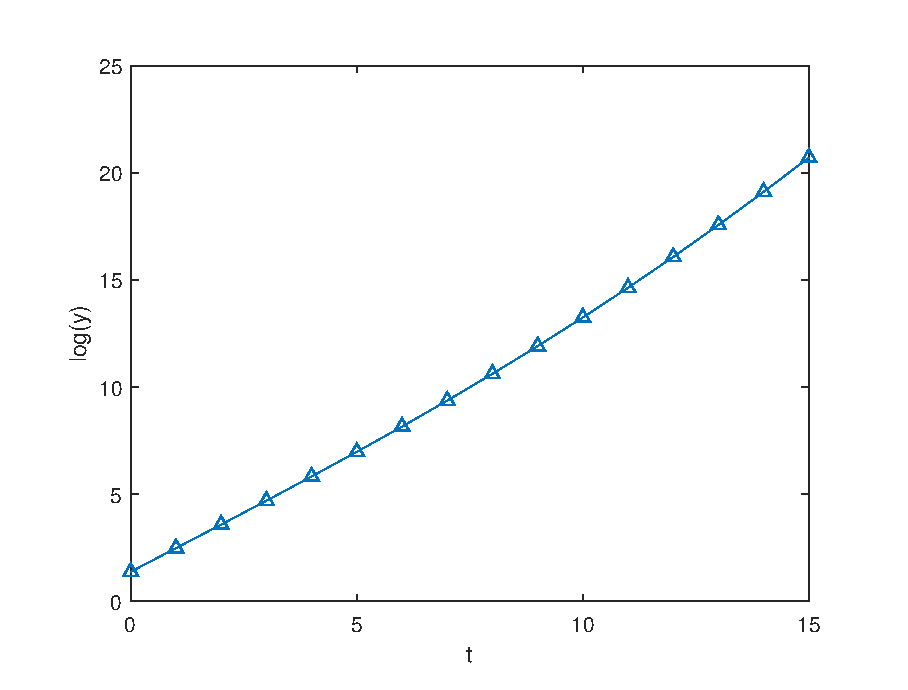
\includegraphics[width=8cm]{../pic/Q3_a.eps}
			\end{figure}
		\item 
			The initial value of $y_k^{(0)}$ is calculated using Euler's method.\\
			Then $y_k^{(i)}$ are calculated in $i-th$ iteration, and the back-ward Euler's method is adopted.
			\begin{equation}
				y_k^{(i)} = y_{k-1}^{(i)} + h \Phi(t_{k}, y_k^{(i-1)})
			\end{equation} 
			The calculation is carried out with matlab, and the results are given as below
			\begin{figure}[!htbp]
				\centering
				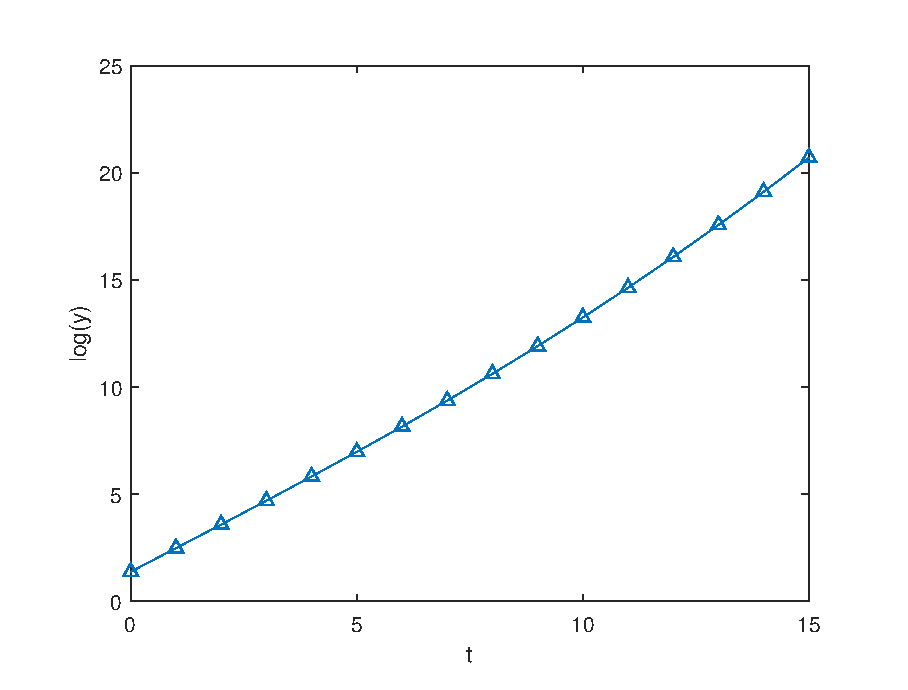
\includegraphics[width=8cm]{../pic/Q3_b.eps}
			\end{figure}
		\item 
			Iteration formula is given as 
			\begin{equation}
				y_k = y_{k-1} + h \Phi(t_{k-1}, y_{k-1}) + \frac{h^2}{2}[\Phi_t(t_{k-1}, y_{k-1}) + \Phi_y(t_{k-1}, y_{k-1}) \Phi(t_{k-1}, y_{k-1})]
			\end{equation}
			The calculation is carried out with matlab, and the results are given as below
			\begin{figure}[!htbp]
				\centering
				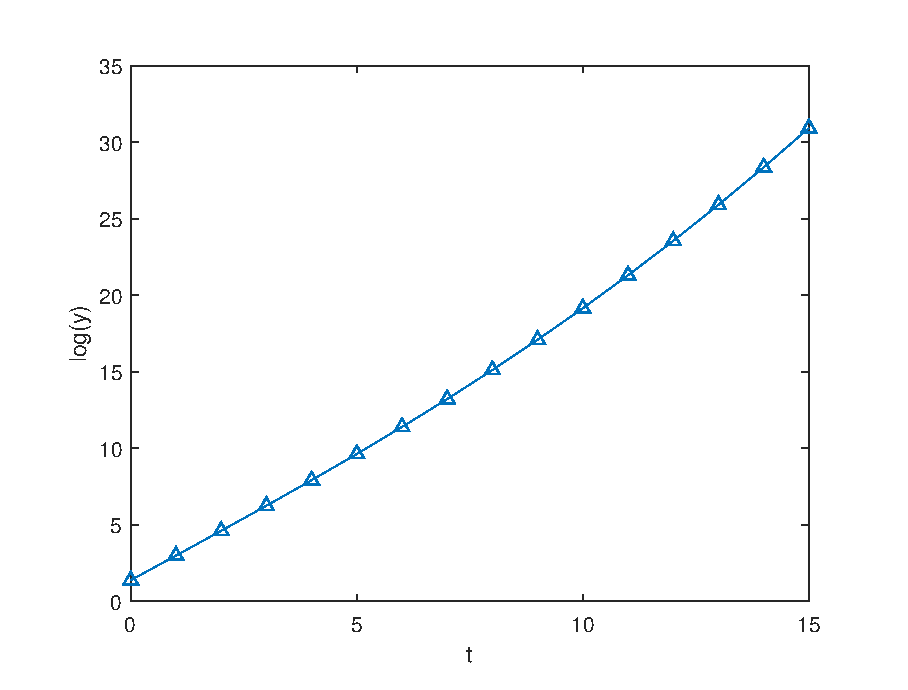
\includegraphics[width=8cm]{../pic/Q3_c.eps}
			\end{figure}
		\item 
			The calculation is carried out with the prediction-correction method. Iteration formulas are given as
			\begin{equation}
				y^* = y_{k-1} + h \Phi(t_{k-1}, y_{k-1})
			\end{equation}
			\begin{equation}
				y_k = y_{k-1} + \frac{h}{2} [\Phi(t_{k-1}, y_{k-1}) + \Phi(t_k, y^*)] 
			\end{equation}
			The calculation is carried out with matlab, and the results are given as below
			\begin{figure}[!htbp]
				\centering
				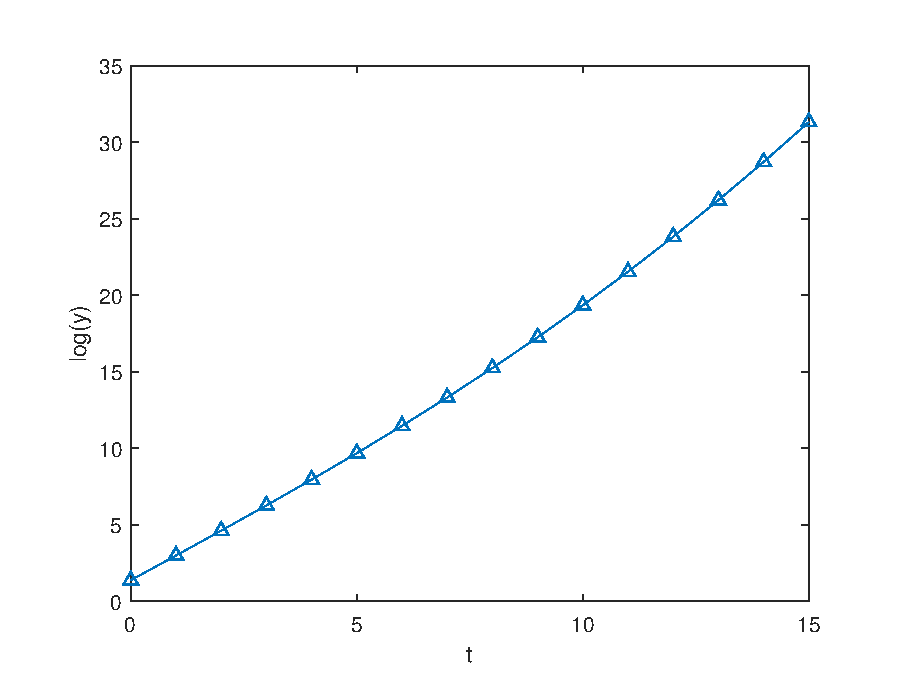
\includegraphics[width=8cm]{../pic/Q3_d.eps}
			\end{figure}
		\item 
			Here, an extra initial point($y_1$) is required, and it is calculated using the Euler's method as
			\begin{equation}
				y_1 = y_0 + h \Phi(t_0, y_0)
			\end{equation}
			Then, the iteration steps are taken as
			\begin{equation}
				y_k = y_{k-1} + \frac{h}{2}[3\Phi(t_{k-1}, y_{k-1}) - \Phi(t_{k-2}, y_{k-2})]
			\end{equation}
			The calculation is carried out with matlab, and the results are given as below
			\begin{figure}[!htbp]
				\centering
				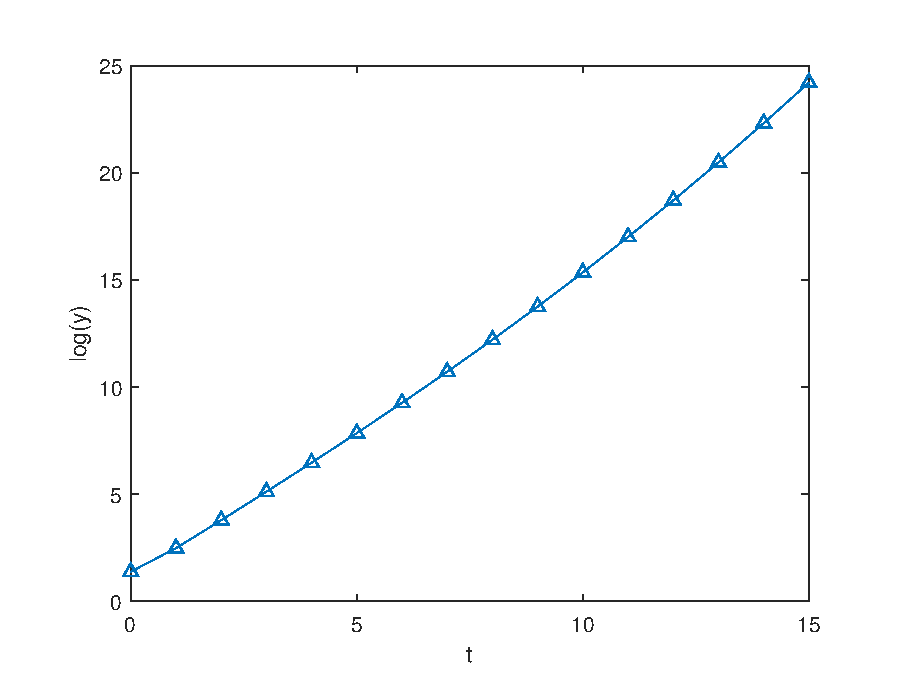
\includegraphics[width=8cm]{../pic/Q3_e.eps}
			\end{figure}
			
	\end{enumerate}

\end{document}